%%%%%%%%%%%%
%
% $Autor: Wings $
% $Datum: 2019-03-05 08:03:15Z $
% $Pfad: Automatisierung/Skript/Produktspezifikation/Powerpoint/AMF.tex $
% $Version: 4250 $
%
%%%%%%%%%%%%


%zusammenführen
\subsection{CIFAR-10 und CIFAR-100}





\subsubsection{Datensatz \ac{cifar}-10}\label{sec:dataset}

Die Datensätze \ac{cifar}-10 und \ac{cifar}-100 sind von Alex Krizhevsky und seinem Team entwickelt   und deshalb nach dem \textbf{C}anadian \textbf{I}nstitute \textbf{f}or \textbf{A}dvanced \textbf{R}esearch\index{Canadian Institute for Advanced Research} benannt worden.  



Der Datensatz \ac{cifar}-10 ist ein Teildatensatz des  Datensatzes \emph{80 Million Tiny Images}. Dieser Teil besteht aus 60.000 Bildern, unterteilt in 50.000 Trainingsbilder und 10.000 Testbilder, welche in 10 Klassen unterteilt und entsprechend gelabelt sind. Die vorhandenen Klassen repräsentieren Flugzeuge, Autos, Vögel, Katzen, Rehe, Hunde, Frösche, Pferde, Schiffe und Lastwagen. Pro Klasse existieren somit 6.000 Bilder, wobei jedes Bild eine Größe von $32\times32$ Pixeln mit drei Farbkanälen hat \cite{Krizhevsky:2009,Krizhevsky:2017}. Ein Auszug des Datensatzes ist in \cref{fig:cifar-example} zu sehen.

\begin{figure}[htb]
	\centering
	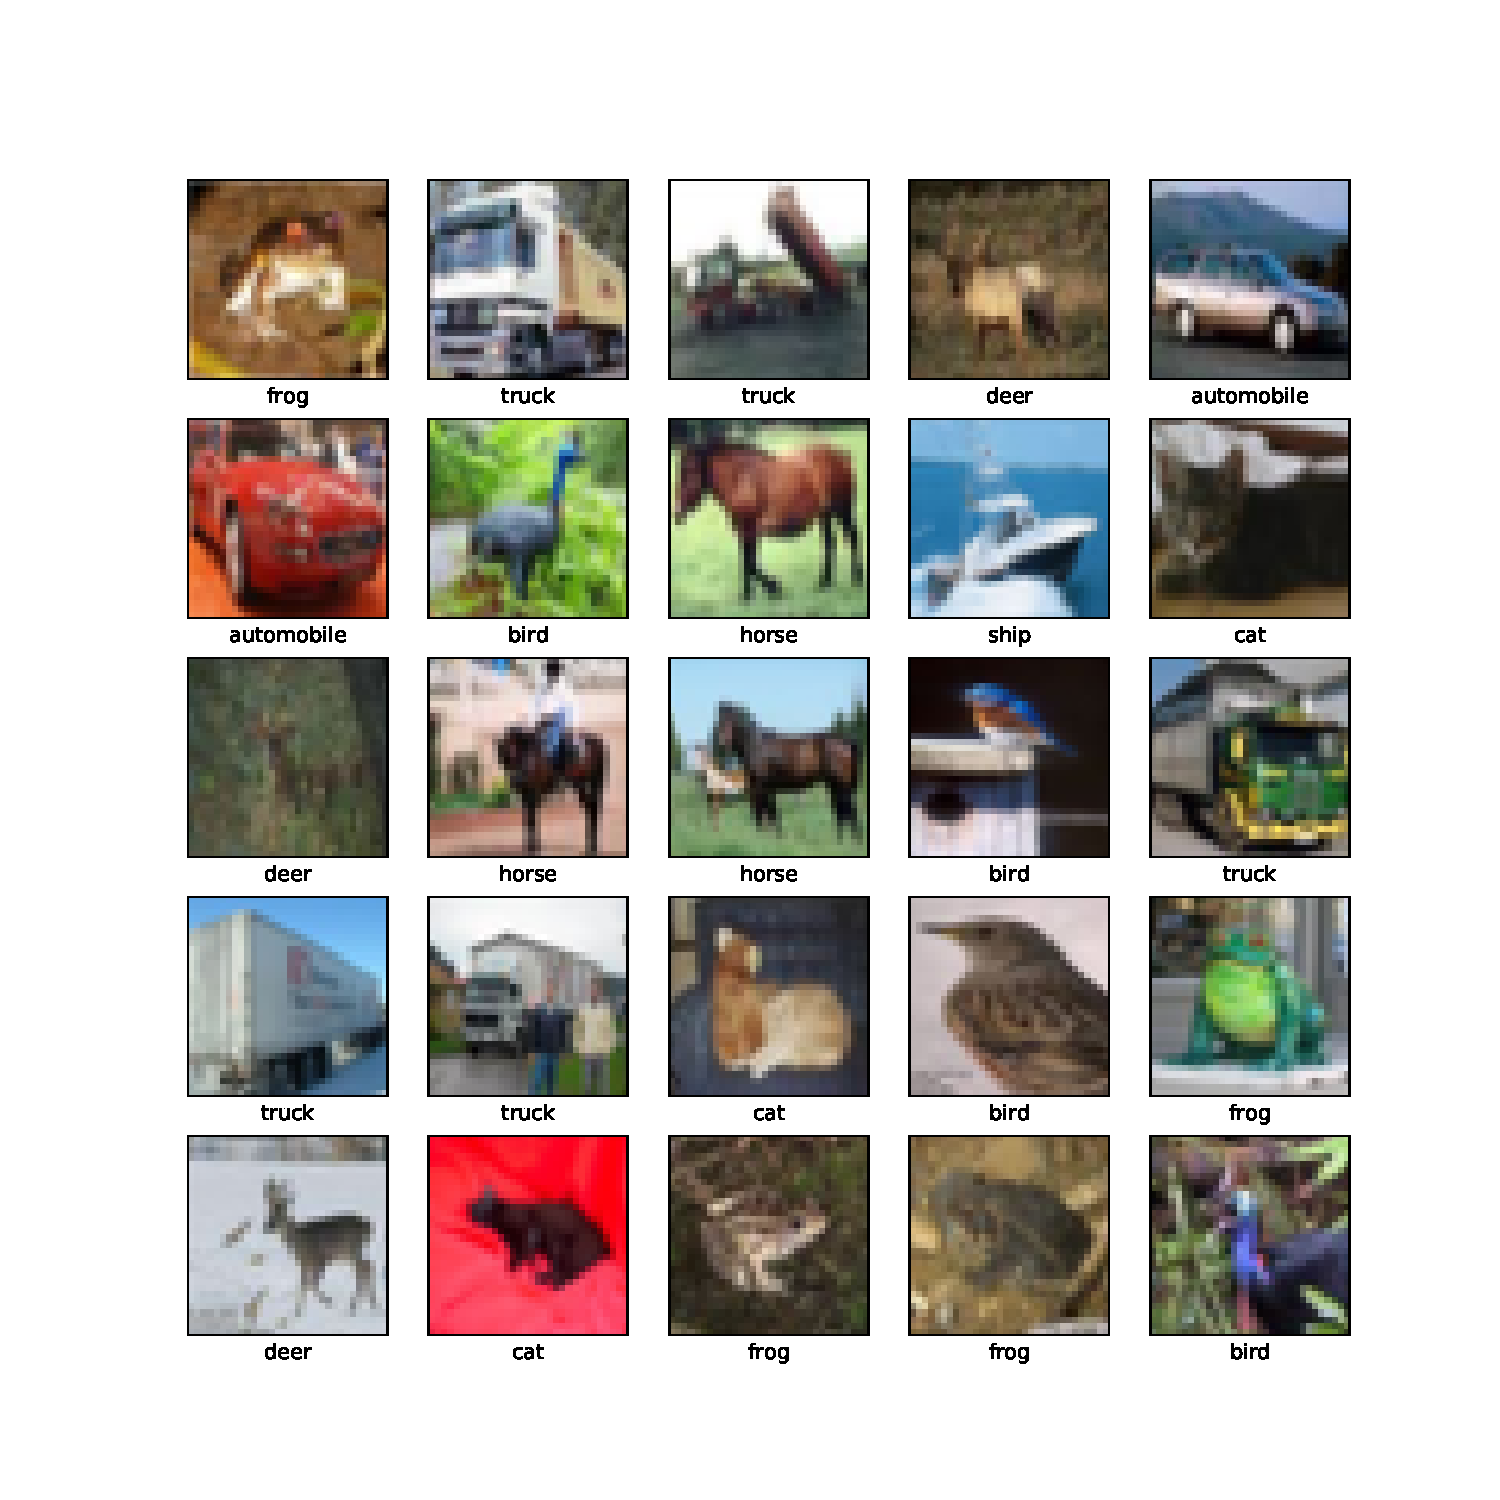
\includegraphics[trim = 25mm 145mm 25mm 15mm, clip, width=\textwidth]{CUDA/cifar-sample.pdf}
	\caption{Auszug von zehn Abbildungen des Datensatz \ac{cifar}-10}
	\label{fig:cifar-example}
\end{figure}

Um den Datensatz in die Python-Umgebung zu importieren, wird hier auf das Modul \python{keras.datasets} zurückgegriffen. Dies beinhaltet eine direkte Schnittstelle zum Datensatz \ac{cifar}-10, welcher durch den Aufruf der Funktion \PYTHON{load\_data()} auf das lokale System heruntergeladen wird. Im Hintergrund wird der Datensatz als gepackte Datei mit der Endung \mytt{.tar.gz} heruntergeladen und im Ordner \FILE{C:\textbackslash Users\textbackslash <Nutzername>\textbackslash .keras\textbackslash datasets} abgelegt. Nach dem Entpacken ist der Datensatz in mehreren serialisierten Objekten enthalten, welche über \PYTHON{pickle} in die Python-Umgebung geladen werden. Daraufhin kann auf die Trainingsdaten, Trainingslabel, Testdaten, und Testlabel über entsprechende Listen zugegriffen werden (\cref{src:cifarimport}). Um bei dem späteren Training das Vanishing-Gradient-Problem zu reduzieren \cite{Ide:2017}, werden die im Datensatz abgelegten RGB-Farbwerte mit dem Wertebereich von 9 bis 255 in Werte von 0 bis 1 umgerechnet. Das Listing~\ref{src:cifarimport} zeigt das Laden und Normalisieren der Daten.


\begin{code}
\begin{lstlisting}[language=MyPython, numbers=left,label={src:cifarimport}]
	(TRAIN_IMAGES, TRAIN_LABELS), (TEST_IMAGES, TEST_LABELS) =  datasets.cifar10.load_data()
	TRAIN_IMAGES = TRAIN_IMAGES / 255.0
	TEST_IMAGES  = TEST_IMAGES / 255.0
\end{lstlisting}
  \caption{Laden und Normalisieren des Datensatzes \ac{cifar}-10}
\end{code}


\subsubsection{Datensatz \ac{cifar}-100}\label{sec:dataset}


Der Datensatz \ac{cifar}-100 hingegen enthält zwar ebenfalls 60.000 Bilder, jedoch unterteilt in 100 Kategorien mit je 600 Bildern. Dabei gibt es zusätzlich 20 Oberkategorien, denen jeweils fünf der 100 Kategorien zugeordnet sind; siehe Tabelle~\ref{TabCIF100}.

\begin{figure}
    \begin{tabular} {l l} 
        \hline
        Superclass &	Classes\\
        \hline
        aquatic mammals & 	beaver, dolphin, otter, seal, whale\\
        fish & 	aquarium fish, flatfish, ray, shark, trout\\
        flowers & 	orchids, poppies, roses, sunflowers, tulips\\
        food containers &	bottles, bowls, cans, cups, plates\\
        fruit and vegetables &	apples, mushrooms, oranges, pears, sweet peppers\\
        household electrical devices &	clock, computer keyboard, lamp, telephone, television\\
        household furniture &	bed, chair, couch, table, wardrobe\\
        insects &	bee, beetle, butterfly, caterpillar, cockroach\\
        large carnivores &	bear, leopard, lion, tiger, wolf\\
        large man-made outdoor things &	bridge, castle, house, road, skyscraper\\
        large natural outdoor scenes &	cloud, forest, mountain, plain, sea\\
        large omnivores and herbivores &	camel, cattle, chimpanzee, elephant, kangaroo\\
        medium-sized mammals &	fox, porcupine, possum, raccoon, skunk\\
        non-insect invertebrates &	crab, lobster, snail, spider, worm\\
        people &	baby, boy, girl, man, woman\\
        reptiles &	crocodile, dinosaur, lizard, snake, turtle\\
        small mammals &	hamster, mouse, rabbit, shrew, squirrel\\
        trees &	maple, oak, palm, pine, willow\\
        vehicles 1 &	bicycle, bus, motorcycle, pickup truck, train\\
        vehicles 2 &	lawn-mower, rocket, streetcar, tank, tractor\\
    \end{tabular}
    \caption{Oberkategorien und Kategorien in \ac{cifar}-100 mit den Originalbezeichnungen}
    \label{TabCIF100}
    
\end{figure}


Der Datensatz kann ebenfalls heruntergeladen und direkt über Keras in TensorFlow importiert werden \cite{kaggle.21.09.2020}:

\begin{code}
    
\begin{lstlisting}[language=MyPython, numbers=left,label={src:cifarimport}]
    import tensorflow as tf
    from tensorflow.keras import datasets
    
    (TRAIN_IMAGES100, TRAIN_LABELS100), (TEST_IMAGES100, TEST_LABELS100) = tf.keras.datasets.cifar100.load_data()
	TRAIN_IMAGES100 = TRAIN_IMAGES100 / 255.0
    TEST_IMAGES100  = TEST_IMAGES100 / 255.0
    
\end{lstlisting}
  \caption{Laden und Normalisieren des Datensatzes \ac{cifar}-100}
\end{code}

